% (find-LATEX "2021-1-C3-curvas-de-nivel.tex")
% (defun c () (interactive) (find-LATEXsh "lualatex -record 2021-1-C3-curvas-de-nivel.tex" :end))
% (defun C () (interactive) (find-LATEXsh "lualatex 2021-1-C3-curvas-de-nivel.tex" "Success!!!"))
% (defun D () (interactive) (find-pdf-page      "~/LATEX/2021-1-C3-curvas-de-nivel.pdf"))
% (defun d () (interactive) (find-pdftools-page "~/LATEX/2021-1-C3-curvas-de-nivel.pdf"))
% (defun e () (interactive) (find-LATEX "2021-1-C3-curvas-de-nivel.tex"))
% (defun o () (interactive) (find-LATEX "2021-1-C3-curvas-de-nivel.tex"))
% (defun u () (interactive) (find-latex-upload-links "2021-1-C3-curvas-de-nivel"))
% (defun v () (interactive) (find-2a '(e) '(d)))
% (defun d0 () (interactive) (find-ebuffer "2021-1-C3-curvas-de-nivel.pdf"))
% (defun cv () (interactive) (C) (ee-kill-this-buffer) (v) (g))
%          (code-eec-LATEX "2021-1-C3-curvas-de-nivel")
% (find-pdf-page   "~/LATEX/2021-1-C3-curvas-de-nivel.pdf")
% (find-sh0 "cp -v  ~/LATEX/2021-1-C3-curvas-de-nivel.pdf /tmp/")
% (find-sh0 "cp -v  ~/LATEX/2021-1-C3-curvas-de-nivel.pdf /tmp/pen/")
%     (find-xournalpp "/tmp/2021-1-C3-curvas-de-nivel.pdf")
%   file:///home/edrx/LATEX/2021-1-C3-curvas-de-nivel.pdf
%               file:///tmp/2021-1-C3-curvas-de-nivel.pdf
%           file:///tmp/pen/2021-1-C3-curvas-de-nivel.pdf
% http://angg.twu.net/LATEX/2021-1-C3-curvas-de-nivel.pdf
% (find-LATEX "2019.mk")
% (find-CN-aula-links "2021-1-C3-curvas-de-nivel" "3" "c3m211cn" "c3cn")
%
% Videos:
% «video-1»  (to ".video-1")
% (find-ssr-links "c3m211cn" "2021-1-C3-curvas-de-nivel" "mrNyBAMOyqo")
% (code-video     "c3m211cnvideo" "$S/http/angg.twu.net/eev-videos/2021-1-C3-curvas-de-nivel.mp4")
% (find-c3m211cnvideo "0:00")
%
% «video-2»  (to ".video-2")
% (find-ssr-links "c3m211cn2" "2021-1-C3-curvas-de-nivel-2" "usBNtNyZRCA")
% (code-video "c3m211cn2video" "$S/http/angg.twu.net/eev-videos/2021-1-C3-curvas-de-nivel-2.mp4")
% (find-c3m211cn2video "0:00" "Derivadas parciais no olhômetro")



% «.video-1»		(to "video-1")
% «.video-2»		(to "video-2")
%
% «.defs»		(to "defs")
% «.title»		(to "title")
% «.links»		(to "links")
% «.exercicio-1»	(to "exercicio-1")
% «.exercicio-2»	(to "exercicio-2")
% «.exercicio-2-cont»	(to "exercicio-2-cont")
% «.exercicio-3»	(to "exercicio-3")
% «.exercicio-3-a»	(to "exercicio-3-a")
%
% «.djvuize»		(to "djvuize")

\documentclass[oneside,12pt]{article}
\usepackage[colorlinks,citecolor=DarkRed,urlcolor=DarkRed]{hyperref} % (find-es "tex" "hyperref")
\usepackage{amsmath}
\usepackage{amsfonts}
\usepackage{amssymb}
\usepackage{pict2e}
\usepackage[x11names,svgnames]{xcolor} % (find-es "tex" "xcolor")
\usepackage{colorweb}                  % (find-es "tex" "colorweb")
%\usepackage{tikz}
%
% (find-dn6 "preamble6.lua" "preamble0")
%\usepackage{proof}   % For derivation trees ("%:" lines)
%\input diagxy        % For 2D diagrams ("%D" lines)
%\xyoption{curve}     % For the ".curve=" feature in 2D diagrams
%
\usepackage{edrx15}               % (find-LATEX "edrx15.sty")
\input edrxaccents.tex            % (find-LATEX "edrxaccents.tex")
\input edrxchars.tex              % (find-LATEX "edrxchars.tex")
\input edrxheadfoot.tex           % (find-LATEX "edrxheadfoot.tex")
\input edrxgac2.tex               % (find-LATEX "edrxgac2.tex")
%
%\usepackage[backend=biber,
%   style=alphabetic]{biblatex}            % (find-es "tex" "biber")
%\addbibresource{catsem-slides.bib}        % (find-LATEX "catsem-slides.bib")
%
% (find-es "tex" "geometry")
\usepackage[a6paper, landscape,
            top=1.5cm, bottom=.25cm, left=1cm, right=1cm, includefoot
           ]{geometry}
%
\begin{document}

%\catcode`\^^J=10
%\directlua{dofile "dednat6load.lua"}  % (find-LATEX "dednat6load.lua")

% %L dofile "edrxtikz.lua"  -- (find-LATEX "edrxtikz.lua")
% %L dofile "edrxpict.lua"  -- (find-LATEX "edrxpict.lua")
% \pu

% «defs»  (to ".defs")
% (find-LATEX "edrx15.sty" "colors-2019")
\long\def\ColorRed   #1{{\color{Red1}#1}}
\long\def\ColorViolet#1{{\color{MagentaVioletLight}#1}}
\long\def\ColorViolet#1{{\color{Violet!50!black}#1}}
\long\def\ColorGreen #1{{\color{SpringDarkHard}#1}}
\long\def\ColorGreen #1{{\color{SpringGreenDark}#1}}
\long\def\ColorGreen #1{{\color{SpringGreen4}#1}}
\long\def\ColorGray  #1{{\color{GrayLight}#1}}
\long\def\ColorGray  #1{{\color{black!30!white}#1}}
\long\def\ColorBrown #1{{\color{Brown}#1}}
\long\def\ColorBrown #1{{\color{brown}#1}}
\long\def\ColorOrange#1{{\color{orange}#1}}

\long\def\ColorShort #1{{\color{SpringGreen4}#1}}
\long\def\ColorLong  #1{{\color{Red1}#1}}

\def\frown{\ensuremath{{=}{(}}}
\def\True {\mathbf{V}}
\def\False{\mathbf{F}}
\def\D    {\displaystyle}

\def\drafturl{http://angg.twu.net/LATEX/2021-1-C3.pdf}
\def\drafturl{http://angg.twu.net/2021.1-C3.html}
\def\draftfooter{\tiny \href{\drafturl}{\jobname{}} \ColorBrown{\shorttoday{} \hours}}



%  _____ _ _   _                               
% |_   _(_) |_| | ___   _ __   __ _  __ _  ___ 
%   | | | | __| |/ _ \ | '_ \ / _` |/ _` |/ _ \
%   | | | | |_| |  __/ | |_) | (_| | (_| |  __/
%   |_| |_|\__|_|\___| | .__/ \__,_|\__, |\___|
%                      |_|          |___/      
%
% «title»  (to ".title")
% (c3m211cnp 1 "title")
% (c3m211cna   "title")

\thispagestyle{empty}

\begin{center}

\vspace*{1.2cm}

{\bf \Large Cálculo 3 - 2021.1}

\bsk

Aula 8: curvas de nível e diagramas de numerozinhos

\bsk

Eduardo Ochs - RCN/PURO/UFF

\url{http://angg.twu.net/2021.1-C3.html}

\end{center}

\newpage

% «links»  (to ".links")
% (c3m211cnp 2 "links")
% (c3m211cna   "links")

Links:

\msk

Sobre ``adivinhar trajetórias'':

{\footnotesize

% (c3m211vtp 6 "sobre-adivinhar-trajetorias")
% (c3m211vta   "sobre-adivinhar-trajetorias")
% http://angg.twu.net/LATEX/2021-1-C3-vetor-tangente.pdf#page=6
\url{http://angg.twu.net/LATEX/2021-1-C3-vetor-tangente.pdf\#page=6}

}

\msk

Diagramas de numerozinhos (2020.2):

{\footnotesize

% (c3m202rcadeia1p 14 "exercicio-6")
% (c3m202rcadeia1a    "exercicio-6")
% http://angg.twu.net/LATEX/2020-2-C3-rcadeia1.pdf#page=14
\url{http://angg.twu.net/LATEX/2020-2-C3-rcadeia1.pdf\#page=14}

}

\msk

Mini-teste sobre cortes em superfícies no olhômetro (2020.2):

{\footnotesize

% (c3m202mt1p 4 "figura-intro")
% (c3m202mt1a   "figura-intro")
% http://angg.twu.net/LATEX/2020-2-C3-MT1.pdf#page=4
\url{http://angg.twu.net/LATEX/2020-2-C3-MT1.pdf\#page=4}

}


\msk

Questão 1 da P1 de 2020.2:

{\footnotesize

% (c3m202p1p 8 "gabarito-1")
% (c3m202p1a   "gabarito-1")
% http://angg.twu.net/LATEX/2020-2-C3-P1.pdf#page=8
\url{http://angg.twu.net/LATEX/2020-2-C3-P1.pdf\#page=8}

}

\newpage

% «exercicio-1»  (to ".exercicio-1")
% (c3m211cnp 3 "exercicio-1")
% (c3m211cna   "exercicio-1")

{\bf Exercício 1.}

Sejam:
%
$$\begin{array}{rcl}
  f(x) &=& x-2 \\
  g(x) &=& 6-x \\
  h(x) &=& \min(f(x), g(x)) \\
  w(x) &=& \max(h(x), 0) \\
  [5pt]
  V(x,y) &=& w(x) \\
  H(x,y) &=& w(y) \\
  P(x,y) &=& \min(V(x,y), H(x,y)) \\
  C(x,y) &=& \max(V(x,y), H(x,y)) \\
  \end{array}
$$

a) Faça os gráficos de $f(x)$, $g(x)$, $h(x)$, $w(x)$.

(Dica: isto é bem parecido com a questão 1 da P1 de 2020.2).

b) Faça os diagramas de numerozinhos de $V(x,y)$, $H(x,y)$,

$P(x,y)$, $C(x,y)$.

\newpage

{\bf Exercício 1 (cont.)}

\msk

Represente graficamente, em 3D com perspectiva improvisada,

as superfícies abaixo. Isto é bem parecido com a questão 1f

da P1 de 2020.2.

\msk

c) $z = V(x,y)$

d) $z = H(x,y)$

e) $z = P(x,y)$

f) $z = C(x,y)$

\newpage

% «exercicio-2»  (to ".exercicio-2")
% (c3m211cnp 5 "exercicio-2")
% (c3m211cna   "exercicio-2")

{\bf Exercício 2.}

Sejam $S_V$, $S_H$, $S_P$ e $S_C$ estas superfícies,

e $X(x_0)$, $Y(y_0)$, $Z(z_0)$ estes planos:
%
$$\begin{array}{rcl}
  S_V &=& \setofxyzst{z = V(x,y)}, \\
  S_H &=& \setofxyzst{z = H(x,y)}, \\
  S_P &=& \setofxyzst{z = P(x,y)}, \\
  S_C &=& \setofxyzst{z = C(x,y)}, \\
  X(x_0) &=& \setofxyzst{x=x_0}, \\
  Y(y_0) &=& \setofxyzst{y=y_0}, \\
  Z(z_0) &=& \setofxyzst{z=z_0}, \\
  \end{array}
$$ 

\newpage

% «exercicio-2-cont»  (to ".exercicio-2-cont")
% (c3m211cnp 6 "exercicio-2-cont")
% (c3m211cna   "exercicio-2-cont")

{\bf Exercício 2 (cont.)}

Represente graficamente em perspectiva improvisada:

a) $S_P∩Z(1)$,

b) $S_C∩Z(1)$,

d) $S_V∩Z(1)$,

e) $S_V∩Z(1)$,

\msk

Agora desenhe num gráfico só a superfície $S_P$

e estes quatro cortes:

f) $S_P∩X(3)$,

g) $S_P∩X(4)$,

h) $S_P∩Y(4)$,

i) $S_P∩Z(1)$.

\msk

Dica: os itens f, g, h e i são parecidos com este mini-teste:

{\footnotesize

% (c3m202mt1p 7 "gabarito")
% (c3m202mt1    "gabarito")
% http://angg.twu.net/LATEX/2020-2-C3-MT1.pdf

\url{http://angg.twu.net/LATEX/2020-2-C3-MT1.pdf}

}



\newpage

% «exercicio-3»  (to ".exercicio-3")
% (c3m211cnp 7 "exercicio-3")
% (c3m211cna   "exercicio-3")

{\bf Exercício 3.}

Este é um exercício pra fazer todo olhômetro, só olhando pras

figuras que você já fez --- os diagramas de numerozinhos e as

figuras 3D. {\sl Se você não conseguir tente de novo, descanse,

tente mais uma vez, repita, etc --- e discuta com os seus

colegas!}

\bsk

Vídeo sobre o exercício 3:

{\footnotesize

% http://angg.twu.net/eev-videos/2021-1-C3-curvas-de-nivel-2.mp4
\url{http://angg.twu.net/eev-videos/2021-1-C3-curvas-de-nivel-2.mp4}

% https://www.youtube.com/watch?v=usBNtNyZRCA
\url{https://www.youtube.com/watch?v=usBNtNyZRCA}

}

\msk

Figuras que eu usei no vídeo:

$
% (find-latexscan-links "C3" "20210716_R2")
% (find-xpdf-page "~/LATEX/2021-1-C3/20210716_R2.pdf")
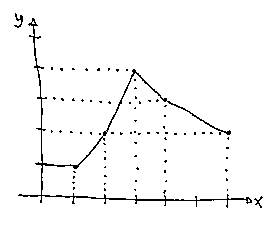
\includegraphics[height=2cm]{2021-1-C3/20210716_R2.pdf}
%
\quad
%
% (find-latexscan-links "C3" "20210716_piramide_2")
% (find-xpdf-page "~/LATEX/2021-1-C3/20210716_piramide_2.pdf")
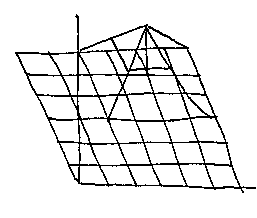
\includegraphics[height=2cm]{2021-1-C3/20210716_piramide_2.pdf}
%
\quad
%
% (find-latexscan-links "C3" "20210716_piramide_1")
% (find-xpdf-page "~/LATEX/2021-1-C3/20210716_piramide_1.pdf")
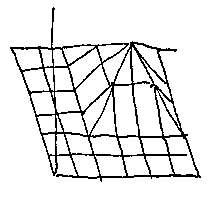
\includegraphics[height=2cm]{2021-1-C3/20210716_piramide_1.pdf}
$




\newpage


\newpage

% «exercicio-3-a»  (to ".exercicio-3-a")
% (c3m211cnp 8 "exercicio-3-a")
% (c3m211cna   "exercicio-3-a")

{\bf Exercício 3 (cont.)}

\msk

Considere a superfície em que $z=P(x,y)$.

\msk

\def\z#1{${}_#1$}

a\z0) Digamos que $(x_0,y_0)=(3,4)$. Quanto é $z$ neste ponto?

\msk

a\z1) Digamos que $(x_1,y_1) = (x_0+0.1,y_0)$; ou seja a gente andou

0.1 pra direita. Quanto é $z$ neste ponto?

\msk

a\z2) Digamos que $(x_2,y_2) = (x_0,y_0+0.1)$; ou seja a gente andou

0.1 pra cima a partir de $(x_0,y_0)$. Quanto é $z$ neste ponto?

\msk

a\z3) Digamos que $(x_3,y_3) = (x_0+0.1,y_0+0.1)$. dá pra chegar

nele a partir de $(x_1,y_1)$ andando 0.1 pra cima, e também dá

pra chegar nele a partir de $(x_2,y_2)$ andando 0.1 pra direita.

Quanto vale $z$ em $(x_3,y_3)$?


\newpage

{\bf Exercício 3 (cont.)}

\msk

Considere a superfície em que $z=P(x,y)$.

\msk

\def\z#1{${}_#1$}

b\z0) Digamos que $(x_0,y_0)=\ColorRed{(4,3)}$. Quanto é $z$ neste ponto?

\msk

b\z1) Digamos que $(x_1,y_1) = (x_0+0.1,y_0)$; ou seja a gente andou

0.1 pra direita. Quanto é $z$ neste ponto?

\msk

b\z2) Digamos que $(x_2,y_2) = (x_0,y_0+0.1)$; ou seja a gente andou

0.1 pra cima a partir de $(x_0,y_0)$. Quanto é $z$ neste ponto?

\msk

b\z3) Digamos que $(x_3,y_3) = (x_0+0.1,y_0+0.1)$. dá pra chegar

nele a partir de $(x_1,y_1)$ andando 0.1 pra cima, e também dá

pra chegar nele a partir de $(x_2,y_2)$ andando 0.1 pra direita.

Quanto vale $z$ em $(x_3,y_3)$?


\newpage

{\bf Exercício 4.}

O que você acabou de fazer no exercício 3 costuma ser feito

em linguagem matemática e numa notação bem compacta, como:
%
\def\und#1#2{\underbrace{#1}_{\text{#2}}}
%
$$\und{
    \und{
    (\und{P(\und{x_0+\und{Δx}{deslocamento em $x$},y_0}{ponto novo})}{$z$ novo} -
     \und{P(\und{x_0,y_0}{ponto original})}{$z$ original})
    }{deslocamento em $z$}
    / Δx
   }{taxa de variação}
$$

Agora você vai tentar fazer uma série de itens como

os do exercício 3, mas na notação nova, e fazendo

tudo de cabeça.

\newpage

{\bf Exercício 4 (cont.)}

Calcule \ColorRed{sem escrever nada}:

\msk

a) Digamos que $(x_0,y_0) = (3,4)$ e $Δx=0.1$.

Calcule $(P(x_0+Δx,y_0) - P(x_0,y_0)) / Δx$.

\msk

b) Digamos que $(x_0,y_0) = (3,4)$ e $Δx=\ColorRed{0.2}$.

Calcule $(P(x_0+Δx,y_0) - P(x_0,y_0)) / Δx$.

\msk

c) Digamos que $(x_0,y_0) = (4,3)$ e $Δy=0.1$.

Calcule $(P(x_0,y_0+Δy) - P(x_0,y_0)) / Δy$.

\msk

d) Digamos que $(x_0,y_0) = (4,3)$ e $Δx=0.1$.

Calcule $(P(x_0,y_0+Δy) - P(x_0,y_0)) / Δy$.

\msk





%\printbibliography

\GenericWarning{Success:}{Success!!!}  % Used by `M-x cv'

\end{document}



%  _                
% | |   _   _  __ _ 
% | |  | | | |/ _` |
% | |__| |_| | (_| |
% |_____\__,_|\__,_|
%                   

 (eepitch-lua51)
 (eepitch-kill)
 (eepitch-lua51)
w = function (x) return max(min(x-2, 6-x), 0) end
P = function (x,y) return min(w(x), w(y)) end
C = function (x,y) return max(w(x), w(y)) end
for x=0,6 do print(w(x)) end
for y=6,0,-1 do
  for x=0,6 do
    printf("%d ", P(x,y))
  end
  print()
end

for y=6,0,-1 do
  for x=0,6 do
    printf("%d ", C(x,y))
  end
  print()
end



%  ____  _             _         
% |  _ \(_)_   ___   _(_)_______ 
% | | | | \ \ / / | | | |_  / _ \
% | |_| | |\ V /| |_| | |/ /  __/
% |____// | \_/  \__,_|_/___\___|
%     |__/                       
%
% «djvuize»  (to ".djvuize")
% (find-LATEXgrep "grep --color -nH --null -e djvuize 2020-1*.tex")

 (eepitch-shell)
 (eepitch-kill)
 (eepitch-shell)
# (find-fline "~/2021.1-C3/")
# (find-fline "~/LATEX/2021-1-C3/")
# (find-fline "~/bin/djvuize")

cd /tmp/
for i in *.jpg; do echo f $(basename $i .jpg); done

f () { rm -fv $1.png $1.pdf; djvuize $1.pdf }
f () { rm -fv $1.png $1.pdf; djvuize WHITEBOARDOPTS="-m 1.0" $1.pdf; xpdf $1.pdf }
f () { rm -fv $1.png $1.pdf; djvuize WHITEBOARDOPTS="-m 0.5" $1.pdf; xpdf $1.pdf }
f () { rm -fv $1.png $1.pdf; djvuize WHITEBOARDOPTS="-m 0.25" $1.pdf; xpdf $1.pdf }
f () { cp -fv $1.png $1.pdf       ~/2021.1-C3/
       cp -fv        $1.pdf ~/LATEX/2021-1-C3/
       cat <<%%%
% (find-latexscan-links "C3" "$1")
%%%
}

f 20210716_R2
f 20210716_piramide_1
f 20210716_piramide_2

f 20201213_area_em_funcao_de_theta
f 20201213_area_em_funcao_de_x
f 20201213_area_fatias_pizza



%  __  __       _        
% |  \/  | __ _| | _____ 
% | |\/| |/ _` | |/ / _ \
% | |  | | (_| |   <  __/
% |_|  |_|\__,_|_|\_\___|
%                        
% <make>

 (eepitch-shell)
 (eepitch-kill)
 (eepitch-shell)
# (find-LATEXfile "2019planar-has-1.mk")
make -f 2019.mk STEM=2021-1-C3-curvas-de-nivel veryclean
make -f 2019.mk STEM=2021-1-C3-curvas-de-nivel pdf

% Local Variables:
% coding: utf-8-unix
% ee-tla: "c3cn"
% ee-tla: "c3m211cn"
% End:
